% begin module transformations-horizontal-stretches
\begin{frame}
\ \only<handout:0| -2>{%
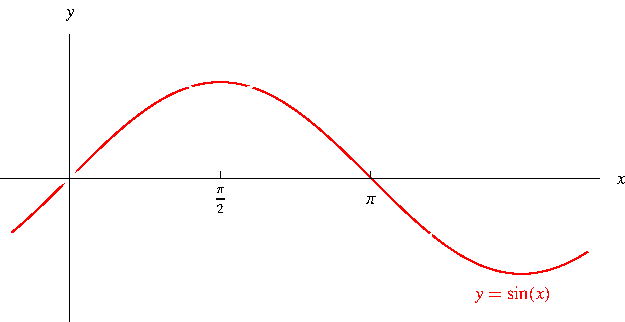
\includegraphics[height=6cm]{precalculus/pictures/01-03-stretcha.pdf}%
}%
\only<handout:0| 3>{%
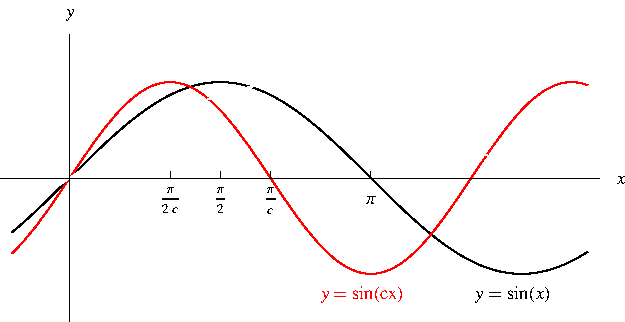
\includegraphics[height=6cm]{precalculus/pictures/01-03-stretchb.pdf}%
}%
\only<4->{%
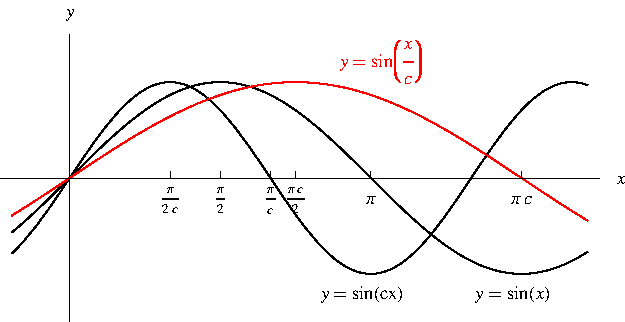
\includegraphics[height=6cm]{precalculus/pictures/01-03-stretchc.pdf}%
}%a

What happens if we multiply or divide $x$ by a constant $c > 1$ before applying $f$?

\uncover<2->{
\begin{tabular}{|l|l|}
\hline
\alert<handout:0| 3>{$f(cx)$} &%
\uncover<3->{\alert<handout:0| 3>{Compress the graph of $f(x)$ horizontally by a factor of $c$.}} \\%
\alert<handout:0| 4>{$f((1/c)x)$} &%
\uncover<4->{\alert<handout:0| 4>{Stretch the graph of $f(x)$ horizontally by a factor of $c$.}} \\%
\hline
\end{tabular}
}
\end{frame}
% end module transformations-horizontal-stretches
